%!TEX root = ../paper.tex

 %\newcommand{\dims}[1]{\langle #1 \rangle}

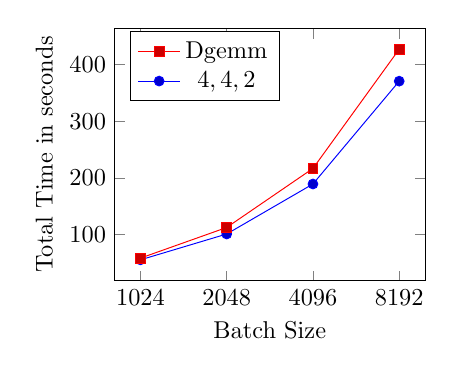
\begin{tikzpicture}[scale=.88]
    \begin{axis}[
        width=.5\textwidth,
        xmode=log,
        log basis x={2},
        xlabel=Batch Size, 
        ylabel=Total Time in seconds,
        legend style={at={(.05,.85)},anchor=west},
        xtick={1024,2048,4096,8192},
        xticklabels={1024,2048,4096,8192},
            /pgf/number format/.cd, 1000 sep={},
            reverse legend,
    ]
    \addplot 
        coordinates {(8192,370.90899634361267) (4096,189.35877895355225)
             (2048,101.08548998832703) (1024,55.47572422027588)};
    \addplot 
        coordinates {(8192,427.3106601238251) (4096,216.82372760772705) 
            (2048,112.62383341789246) (1024,58.5027711391449)};
    \legend{$\dims{4,4,2}$,Dgemm}
    \end{axis}
\end{tikzpicture}